

\section{Summary of Proteome Datasets.}
\label{sec:SI_exp_summary}

Here we provide a brief summary of the experiments behind each proteomic
data sets. The purpose of this section is to better identify the steps taken
by the authors to arrive at absolute protein abundances. In the following
section (Section~\nameref{sec:SI_data_summary}) we will then provide a summary of the
final protein abundance measurements that were used for in the main text.

Table \ref{table:datasets} provides an overview of the main data sets that
we considered. These are predominately mass spectrometry-based,
with the exception of the work from Li \textit{et al.} (2014) which used ribosomal
profiling, and the fluorescence-based counting done in Taniguchi \textit{et al.}
(2010).

\begin{table}[bt]
\caption{\label{tab:datasets}Overview of proteomic data sets.}
% Use "S" column identifier to align on decimal point
\begin{tabular}{l l l }
\toprule
Author & Method & Reported Quantity \\
\midrule
Taniguchi \textit{et al.} (2010)  & YFP-fusion, cell fluorescence    & fg/copies per cell      \\
Valgepea \textit{et al.} (2012)   & mass spectrometry                & fg/copies per cell      \\
Peebo \textit{et al.} (2014)      & mass spectrometry                & fg/copies per fl        \\
Li \textit{et al.} (2014)         & ribosomal profiling              & fg/copies per cell $^a$ \\
Soufi \textit{et al.} (2015)      & mass spectrometry                & fg/copies per cell      \\
Schmidt \textit{et al.} (2016)    & mass spectrometry                & fg/copies per cell $^b$ \\
Caglar \textit{et al.} (2017)     & mass spectrometry                & relative abundance      \\
\bottomrule
\end{tabular}

\medskip
a. The reported values assume that the proteins are long-lived compared to the generation time
but are unable to account for post-translational modifications that may alter absolute protein abundances.
\\
b. This mass spectrometry approach differs substantially from the others since in addition to
the relative proteome-wide abundance measurements, the authors performed absolute quantification of
41 proteins across all growth conditions (see Section~\nameref{sec:SI_schmidt} for more details on this).
\end{table}

\subsection{Fluorescence based measurements of protein abundance}
In the work of \cite{taniguchi2010}, the authors used a chromosomal YFP fusion
library where individual strains have a specific gene tagged with a YFP-coding
sequence. 1018 of 1400 attempted strains were used in their work. For each
strain, a fluorescence microscope was used to collect cellular YFP intensities.
Through automated image analysis, the authors normalized intensity measurments
by cell size to account for the change in size and expression variability across
the cell cycle. YFP intensities were also corrected for cellular
autofluorescence, and final absolute protein levels were determined by a
calibration with single-molecule fluorescence intensities, performed seperately
using a purified YFP solution.

\subsection{Ribosomal profiling measurements of protein abundance}





\subsection{Mass spectrometry measurements of protein abundance}


We begin The general strategy taken in these works is to quantify fractional
abundance of each protein and then to convert these to absolute abundance by
multiplying these fractions by the bulk measured total cellular protein
abundance. Note that the work of Peebo \textit{et al.} (2014) did not perform
any measurement of cell count or volume, and thus were only able to report
cellular protein concentration.

Exceptions to this are found in Schmidt \textit{et al.} and Taniguchi \textit{et al.}.
A key distinction in the work of Schmidt \textit{et al.} is that in addition to
determining relative abundance by mass spectrometry, they also selected 41
enzyme that cover over four orders of magnitude in cellular abundance to use in
absolute protein quantification. Specifically, synthetic peptides were generated
for each of these 41 enzymes and used to provide a calibration between measured
mass spectrometry intensities and absolute protein abundances (using stable
isotope dilution (SID) and selected reaction monitoring (SRM), though the
details of this are beyond the scope of this section). In the work of Taniguchi
\textit{et al.},  the authored tagged each protein with a  yellow fluorescent
protein (YFP) and used fluorescence as readout of cellular expression.



\begin{table}[bt]
\caption{\label{tab:datasets}Overview of proteomic data sets.}
% Use "S" column identifier to align on decimal point
\begin{tabular}{l l l }
\toprule
Author & Method & Reported Quantity \\
\midrule
Measurements  & YFP-fusion, cell fluorescence    & fg/copies per cell      \\
Valgepea \textit{et al.} (2012)   & mass spectrometry                & fg/copies per cell      \\
Peebo \textit{et al.} (2014)      & mass spectrometry                & fg/copies per fl        \\
Li \textit{et al.} (2014)         & ribosomal profiling              & fg/copies per cell $^a$ \\
Soufi \textit{et al.} (2015)      & mass spectrometry                & fg/copies per cell      \\
Schmidt \textit{et al.} (2016)    & mass spectrometry                & fg/copies per cell $^b$ \\
Caglar \textit{et al.} (2017)     & mass spectrometry                & relative abundance      \\
\bottomrule
\end{tabular}

\medskip
a. The reported values assume that the proteins are long-lived compared to the generation time
but are unable to account for post-translational modifications that may alter absolute protein abundances.
\\
b. This mass spectrometry approach differs substantially from the others since in addition to
the relative proteome-wide abundance measurements, the authors performed absolute quantification of
41 proteins across all growth conditions (see Section~\nameref{sec:SI_schmidt} for more details on this).
\end{table}


Figure \ref{} shows the distribution in reported protein abundance for   a  subset
of  the data.

An important consideration is whether the reported abundance per cell are correlated. while
we expect some variability in expression of each protein due to growth rate, the reported
values are nonetheless expected to be correlated. Figure \ref{fig:dataset_correlations} compares each dataset to the copy numbers from Schmidt \textit{et al.}, grown in M9 minimal media supplemented with glucose.
%
% \begin{figure}[H]
% 		\centering
%     \includegraphics[width=1\textwidth]{../../figures/dataset_correlations.pdf}
%   \caption{}
%   \label{fig:dataset_correlations}
% \end{figure}
%
% \begin{figure}[H]
% 		\centering
%     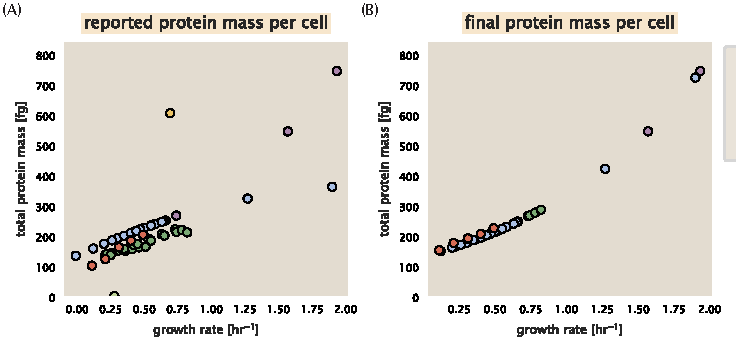
\includegraphics[width=1\textwidth]{../../figures/dataset_corrections.pdf}
%   \caption{}
%   \label{fig:dataset_correlations}
% \end{figure}
%
